%\documentclass[a4paper, twocolumn]{article}
\documentclass[a4paper]{article}
\newcommand{\papertitle}{Potential of I/O-Aware Workflows in Climate and Weather}

\usepackage[a4paper, margin=2cm]{geometry}

\usepackage[utf8]{inputenc}
\usepackage[T1]{fontenc}
\usepackage{graphicx}
\usepackage[english]{babel}
\usepackage[colorlinks=true,urlcolor=red]{hyperref}
\usepackage{url}
\usepackage{float}
\usepackage{cleveref}
\usepackage{todonotes}
\usepackage{comment}
\usepackage{ulem}

\newcommand{\jk}[1]{\todo[inline]{JK: #1}}

\usepackage{multicol}
\setlength{\columnsep}{1cm}

\usepackage{fancyhdr}
\fancyhead{}
\fancyfoot{}
\fancyhead[l]{\papertitle}
\fancyhead[r]{
\includegraphics[height=1em]{esiwacelogo_type_grey_left_2c_ext}}
\fancyfoot[r]{\thepage}
\pagestyle{fancy}
\renewcommand{\headrulewidth}{1pt}
\renewcommand{\footrulewidth}{1pt}

\usepackage{titling}
\pretitle{\begin{center}\Large\bfseries}
\posttitle{\end{center}\vskip 0.5em}

\graphicspath{{./assets/}}

\title{\papertitle}

\author{Julian M. Kunkel
  \textit{University of Reading}
    \and
  Luciana R. Pedro
  \textit{University of Reading}
}
\date{\today}


\begin{document}
\maketitle
\thispagestyle{fancy}

\section*{Abstract}
The efficient, convenient, and robust execution of data-driven workflows and enhanced data management are key for productivity in scientific computing.
\sout{{\color{blue}{
Traditionally, in HPC, the concerns of storage and computing are separated and optimised independently from each other, and, moreover, independently from the needs of end-to-end user workflows that ultimately lead to insight.}}}
{\color{cyan}{
Traditionally, in HPC, the concerns of storage and computing are separated and optimised independently from each other and from the needs of end-to-end user.}}
As climate and weather workflows become increasingly complex and blend beyond data centres while, at the same time, storage hierarchies become deeper, the community investigates means to re-organise storage access to utilise such environments fully.

The key contributions of this paper are:
1) we sketch the visions of an integrated data-driven approach and discuss the challenges and implications of this strategy.
2) we illustrate architecture and roadmap that allows the seamless integration into existing workflows.
The tools employed here to achieve this extended workflow are Cylc, XIOS, DDN IME, and ESDM.

%Basically, we believe workflows composed of data, computing, and communication-intensive tasks should drive the interfaces and hardware configurations to best support the programming models.
From the user perspective, we ultimately aim to provide an abstraction to data dependencies.
The proposed changes increase the opportunity of implementations for smarter scheduling of computing and storage in heterogeneous storage environments considering characteristics of workflows and data.
From the system perspective, the vision aims to derive an execution plan that utilises the available hardware and software infrastructure within a data centre.


\section{Introduction}

High-Performance Computing (HPC) harnesses the fastest hardware components to enable the execution of tightly coupled applications from science and industry.
Typical use-cases cover the numerical simulation of physical systems and the analysis of large-scale observational data.
In the domain of climate and weather, there is a considerable demand for the orchestration of ensembles of simulation models and the generation of data products.
A weather forecast service such as ECMWF generates .... \jk{Cylc team, please provide some facts}
Likewise, ensembles in climate can ...

Based on their needs, the {\color{cyan}{HPC}} community has developed a software ecosystem that supports them to execute their large-scale workflows.
While the current advances correspond to a big leap forward, many processes still require experts.
For example, porting a workflow from one system to another requires to adjust runtime parameters of applications and to decide how data is managed.
Since performance is of crucial importance to large-scale workflows, careful attention must be paid to exploit the system characteristics of the target supercomputer.
To obtain the best performance, a specific supercomputer typically requires substantial changes to the workflow to tailor the workflow to the particular machine.
For instance, a data-driven workflow may benefit from using a heterogeneous set of computing and storage technology at the same time.

Knowing the capabilities, interfaces, and performance characteristics of individual components are mandatory to make the best use of them.
As the complexity of systems increases and alternative storage and computing technologies provide unique characteristics, it becomes increasingly difficult even for experts to manually optimise I/O in workflows. {\color{cyan}{First time I/O is mentioned. I would change to something like... it becomes increasingly difficult even for experts to manually optimise resources (other stuff) and, in particular, I/O in such workflows.}}
In many cases, modifications are not performed because: 1) they are labour intense: any change to the workflow requires careful validation which may not pay off for small scale runs; 2) users are not aware of the potential of the complex system.

In this paper, we show that knowledge about workflow execution and overall experimental design helps to
optimise the execution of climate and weather workflows and may increase the performance, throughput and cost-efficiency of the environments, providing an incentive to users and data-centres that cannot be neglected.

The paper is organised as follows:
In \Cref{sec:workflows}, we provide an overview of the specification of workflows in climate and weather and the involved software stack.

\jk{TODO}


\section{Workflows in Climate/Weather}
\label{sec:workflows}

In this section, we describe how the environment workflows are executed in the typical software stack.

\subsection{Data Center Infrastructure}

To satisfy the needs for different workflows, data centres are providing a infrastructure consisting of computing and storage devices with different characteristics which makes them more efficient for specific tasks.
Take, for example, the supercomputer Mistral at DKRZ that consists of about {\color{cyan}{about?}} 3,000 nodes.
It offers two types of compute nodes equipped with different CPUs and a range of GPU nodes.
Each node provides an SSD for local storage and DKRZ has additionally two shared Lustre file systems with different performance characteristics.
The user can access both file systems \sout{{\color{blue}{as a work and scratch file system}}}. {\color{cyan}{as work and scratch file systems.}}
While data is kept on the work file system indefinitely, its available space is limited by a quota.
The scratch file system allows to store more data, but data is automatically deleted after some time.

Future centres are expected to have even more heterogeneity. A variety of accelerators (GPU, TPU, FPGAs), active storage, in-memory, and in-network computing technologies provide storage and processing capabilities.
\Cref{fig:heterogeneous} shows such an environment with a focus on computation and storage.
Some of these technologies might be local to specific compute nodes or globally available.
Depending on the need, the storage characteristics range from predictable low-latency (in-memory storage, NVMe) to online storage (SSD, HDD), and cheap storage for long-term archival (tape).
\jk{Mention BBs, e.g., DDN IME}
Naturally, the variety of tasks executed by a single workflow may benefit from the different storage and computing infrastructure.

\begin{figure}[H]
  \centering
  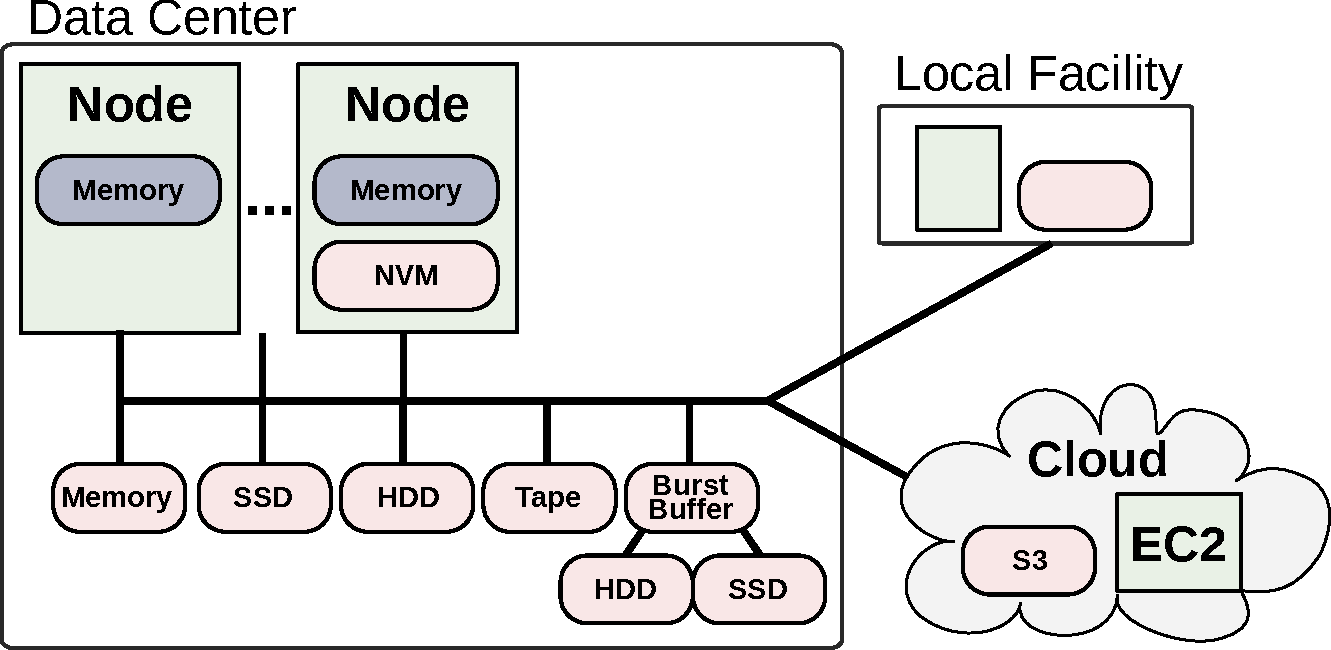
\includegraphics[width=0.6\columnwidth]{system}
  \caption{Example of an heterogeneous HPC landscape}
  \label{fig:heterogeneous}
\end{figure}


\subsection{Software Stack}

The relevant software stack involved in executing workflows is depicted in \Cref{XXX}
\jk{insert picture about software stack here}
To solve a computational problem, we can consider describing the necessary steps from the start to the insight {\color{cyan}{insight? I really don't undestand some of your uses of this word.}} as a workflow.
Cylc executes a workflow description comprising of the individual data processing steps and the dependencies among them.

\subsection{I/O Stack}

A typical I/O stack for a single parallel application like a climate model is shown in \Cref{fig:layers}.

\begin{minipage}{0.2\textwidth}
\begin{figure}[H]
  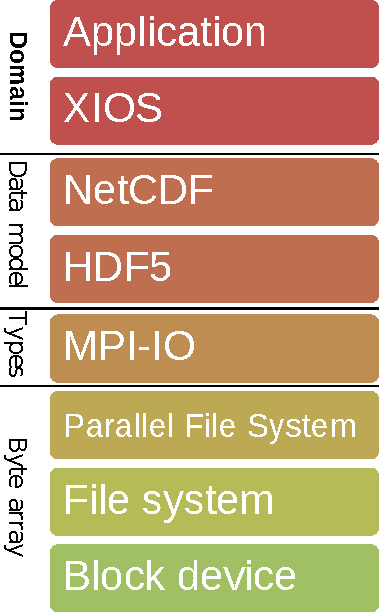
\includegraphics[width=\textwidth]{layers-xios}
  \caption{I/O Path for an MPI-Parallel Application}
  \label{fig:layers}
\end{figure}
\end{minipage}
\qquad
\begin{minipage}{0.7\textwidth}
In our example, we assume the application is parallelised for performance reasons and uses MPI to \sout{{\color{blue}{coordinate}}} {\color{cyan}{run}} the application.
It may use XIOS to gather data from individual fields which then uses NetCDF4 to store the data as a file.
XIOS provides a domain-level semantics and ...\jk{TODO}
Under the hood, NetCDF4 used the HDF5 API and file format.
Internally, HDF5 uses MPI again and its data types to specify the nature of the data stored.
\sout{{\color{blue}{Finally, data is stored on a parallel file system like Lustre, which, on the server-side, stores data in a local file system that is stored on block devices and storage media such as SSDs and HDDs.}}}
{\color{cyan}{Finally, data is stored on a parallel file system like Lustre, which, on the server-side, stores data in local file system as block devices on storage media such as SSDs and HDDs.}}

Different applications involved in a workflow may use a different I/O stack to store their outputs.
Naturally, the application that inputs previously generated data must use a compatible API to be able to read the specific data format.
In this figure, for example, XIOS is beneficial for parallel I/O and a process might directly rely on the NetCDF API to read previous data.
\end{minipage}


\subsection{Cylc}

Cylc is in charge to execute and monitor workflows in which each step is submitted to the batch scheduler of a data centre.
 %, and the relevance of heterogeneous infrastructure to run workflows.
%We focus on high-level considerations to illustrate mandatory concepts.



Consider the Cylc suite configuration for a toy monthly cycling workflow in Figure \ref{fig:cylc}.
In this workflow, a warm-cycled atmospheric model (\textbf{model}) simulates the physics from a current state to predict the future after a timestep, for example, after six hours.
This process is repeated in the model to simulate month and years into the future.
Once the simulation of a month is computed, the data for this month can be analysed.
{\color{cyan}{This is wuite strange for me. It means that only after a month is completed one will use the information to start previsions? I would expect it to be more like a window-month than a fixed month, no?}}
A user has specified a detailed workflow in a Cylc suite file (\texttt{suite.rc}).
In this workflow, the \textbf{model} is followed by postprocessing (\textbf{post}), forecast verification (\textbf{ver}), and product generation (\textbf{prod}) tasks.
Also, consider, in addition, a task \textbf{check} that compares some verification metric against products from two cycles earlier.

\begin{figure}[H]
  \centering
  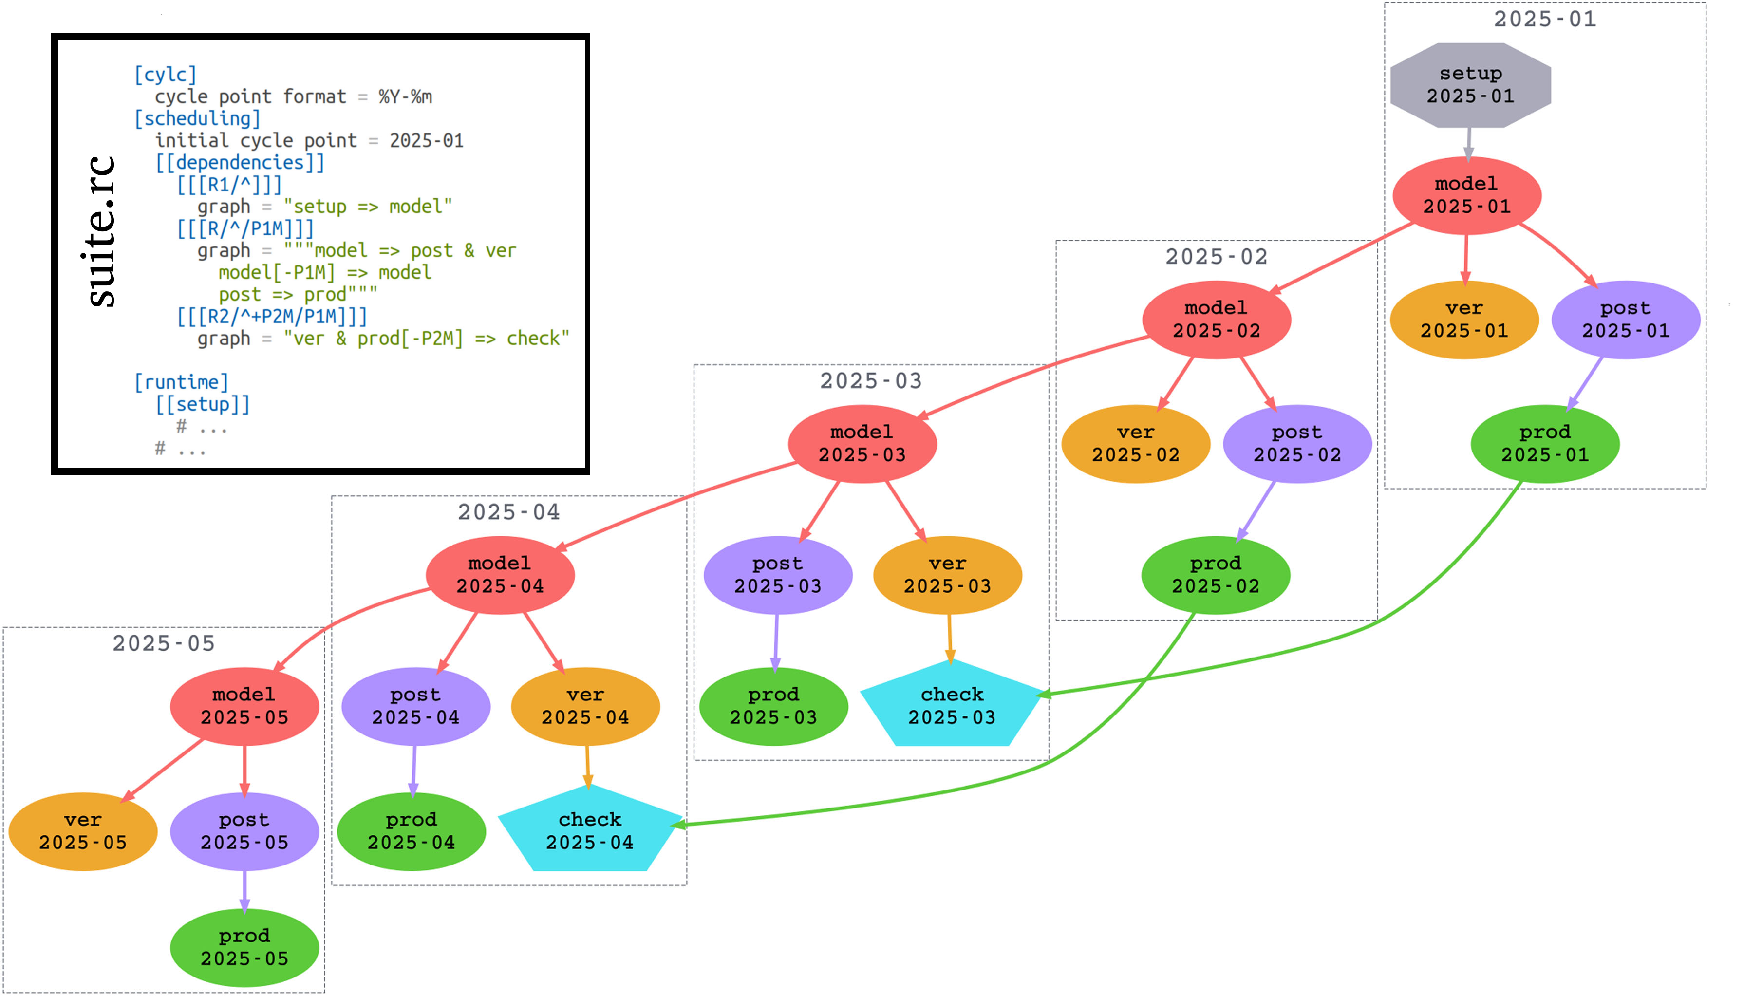
\includegraphics[width=0.9\columnwidth]{cylc1}
  \caption{Example workflow\cite{8675433}}
  \label{fig:cylc}
\end{figure}

This suite presents the dependencies among the tasks, but it is missing the information about I/O and storage.
Decisions about storage must take into consideration the architecture in which the workflow will run.
The developers make the configuration about parallelism and where the data is stored in a script file that is executed for each specific task.

\subsection{Data Management}

The scripts for the tasks in Cylc define how the data is stored on the available storage systems.
\Cref{fig:lifecycle} shows three possible life cycles and the access pattern for a specific dataset.
Consider that the machine has three file systems: a fast \textbf{scratch} file system on which data may reside only for a week, a slower \textbf{work} file system, and each node has a \textbf{local} file system.
As shown in \Cref{fig:lifecycle}(a), the dataset could be stored on the \textbf{local} storage first to avoid congestion on the \textbf{work} file system, then be migrated to \textbf{work} file system where subsequent tasks of the workflow may read it multiple times.
In the end, this dataset might be an intermediate product that can then be deleted.
Alternatively (\Cref{fig:lifecycle}(b)), it could be stored on the \textbf{scratch} file system immediately and accessed there.
However, that would require that the last read access happens before files on \textbf{scratch} are automatically removed.
The last scenario (\Cref{fig:lifecycle}(c)) presents the case where data is created on \textbf{work} by a task, but then it is copied to a \textbf{local} node to allow read accesses of subsequent tasks which might be beneficial for small random accesses.
However, it would require that the subsequent tasks are placed on the same machine where data is now stored.
The scientist responsible for the workflow must optimise the available resources intuitively.
These are just examples and currently the scientists perform such kind of optimisations manually.


\begin{figure}[H]
  \centering
  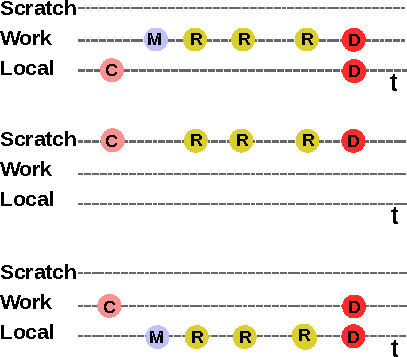
\includegraphics[width=0.6\columnwidth]{lifecycle}
  \caption{Life cycle of one dataset: \textbf{C}reate, \textbf{M}igrate, \textbf{R}ead, and \textbf{D}elete}
  \label{fig:lifecycle}
\end{figure}


\section{State of the Art}

Other tools for workflow handling, how is this information transported?

dataspaces

ADIOS


\section{Vision for I/O-Aware Workflows}

Applied scientists should not spend time understanding hardware characteristics, but using their time to develop their work, let the computer do the job the simplest way as possible, and just collect and analyse the results.
However, nowadays, to be able to run a job in a HPC environment efficiently, researchers have to have profound knowledge about their workflow, which is expected, but also about decisions regarding storage, communication, and computing.

We propose an approach to reduce the burden on researchers and, at the same time, optimise the decisions about jobs running in HPC systems.
Once we have an automated decision about where the job will run and how the storage will be managed, scientists can then run their workflows in any machine without further interactions and even without previous knowledge about the machine architecture.


\subsection{Workflow Description}

So far, Cylc allowed specifying tasks and the dependencies among them.
We aim to enrich this information with characteristics for input, and the products. {\color{cyan}{What?!}}
An example workflow containing data products is illustrated in \Cref{fig:workflow}.
\sout{{\color{blue}{Arrows indicate dependencies between nodes that represent tasks and data.}}}
{\color{cyan}{Nodes represent tasks and data and arrows indicate dependencies among tasks.}}
In the example, Task\,1 needs two datasets to perform its work, it directly communicates with Task\,2 and produces Product\,1.
Most of the workflow can run automatically, except for the manual quality control of the products and the final data usage of Product\,3.
This last step represents the typical uncertainty of data reuse, i.e., it is unclear how Product\,3 will be used further.
In this approach, each task is annotated with the required inputs and the generated products.
Each data product is annotated with metadata such as data life cycle information, e.g., the value of data and how long should it be kept.

\begin{figure}[H]
  \centering
  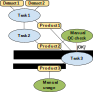
\includegraphics[width=0.4\columnwidth]{workflow}
  \caption{Example of a high-level workflow}
  \label{fig:workflow}
\end{figure}


\subsection{Potential Benefit}



\section{Design}
What changes now in terms of specification?

\subsection{User Perspective Workflow}

From the user perspective, the workflow can be described by the following categories:

\begin{description}

\item[Input] The information inserted in the workflow. It is composed of datasets describing, for instance:

\begin{itemize}

\item The actual input data, for instance, the dates for the experiments, how many times the workflow has to run, etc.

\item The dependencies among the tasks.

\item The I/O information, i.e., where the datasets will be stored in each step of the workflow.

\item The information about the lifetime of the final outcome.

\item The steps in which manual decisions have to be made.

\end{itemize}

For simplicity, we will call these datasets as \texttt{input.ds}.

\item[Task 1] The task is specified by the user and the information we have about it is:

\begin{itemize}

\item The data input.

\item The data output.

\item How long the data has to be stored.

\item The dependencies regarding the other tasks.

\end{itemize}

In the case of Task 1, we have:

\begin{itemize}

\item Task\,1 has no prior dependencies other than the general input.

\item Task\,1 is a dependency for running Task\,2 and Task\,3.

\item For simplification purposes, we will assume that Task\,1 has the datasets \texttt{input1.ds}, \texttt{output1.ds}, and \texttt{storage1.ds} as descriptors.

\end{itemize}

\item[Task 2]

\begin{itemize}

\item Task\,2 is dependent on the outcomes of Task\,1.

\item Task\,2 has the datasets \texttt{input2.ds}, \texttt{output2.ds}, and \texttt{storage2.ds} as descriptors.

\end{itemize}

\item[Task 3]

\begin{itemize}

\item Task 3 dependent on the outcomes of Task\,1 and Task\,2. It does not require any other task to be started and, after finished, no other task will use its results other than the overall output.

\item Task 3 has the datasets \texttt{input3.ds}, \texttt{output3.ds}, and \texttt{storage3.ds} as descriptors.

\end{itemize}

\item[Product]

A product is any of the possible outcomes of a task. Usually is composed of datasets that will be used by other tasks or generate the final output.

\item[Final Output]

The final output consists of all datasets generated by the workflow. Those datasets have to be stored for a specific amount of time previously described in one of the input datasets.

For simplicity, we will call these datasets as \texttt{output-workflow.ds}. In this specific example, it is composed by the datasets \texttt{output1.ds}, \texttt{output2.ds}, and \texttt{output3.ds}.

\end{description}

For this work, the datasets belonging to \texttt{input-workflow.ds} are the datasets inserted as input for the running Cylc. The Cylc tool receives, as predefined, information about the storage and dependencies of the datasets. This information is used to construct and run the complete workflow, but it is not used to optimise intermediate steps.
The configuration is already predefined, and it cannot change. For instance, if it is established that Task\,2 depends on Task\,1, then we have to wait for Task\,1 to be completed to start running Task\,2.
But several options can be optimised if we know the whole workflow in advance. Thinking what about I/O, for instance, no decision is being made about an optimal way to store the data. Consider, as an example, that the datasets from \texttt{output1.ds} are divided into \texttt{output1-final.ds} and \texttt{output1-task2.ds}. Then, it is clear that \texttt{output1-task2.ds} will be required to run Task\,2, and, because of that, should be put in fast storage to quickly being retrieved, or even kept in local storage. The \texttt{output1-final.ds} dataset, however, can go directly to tape, if the lifetime of the final output has to be stored for a long time, but no access is required from the current workflow.

Those simple examples are here to demonstrate that, once we have the complete knowledge about how the workflow is expected to run, we can optimise steps that were before predefined by the user usually considering only options for feasibility. The user input is one of the viable options to run the workflow, but probably it is not the best, assuming other options are available. The user might even have analysed other options, but s/he has naively done that (usually by trial and error). By automating these tasks, specifically a smarter route for the tasks taking into consideration the architecture available and the way the datasets are stored during the intermediate steps of the workflow, we have a twofold gain:

\begin{itemize}

\item The user does not have to worry about the architecture that the workflow will use, removing from the specialist the decision-making process; and

\item The workflow will be optimised for the specific workflow without extra input from the user and the resources will, then, be better utilised.

\end{itemize}

In this paper, we approach two ways to have the extra information from the user to be able to make decisions about storage and the processing of the datasets/tasks.

\begin{itemize}

\item The user will insert this information as an additional file to the Cylc workflow management. In fact, the user is already doing that, but he is doing that in just one specific way, to make the workflow possible. Here, we are thinking about simplifying the information the user is already providing. So, instead of giving the complete workflow to Cylc, we are expecting the user to provide straightforward information, like:

\begin{itemize}

\item Task 1 usually requires ten hours running in a pc with standard configuration\footnote{Intel Core i5, 8 GB RAM, and 500 GB internal storage drive, for instance.}, requires 100 GB of storage that has to be persistent for no more than one week.

\item Task 2 usually requires two hours running in a pc with standard configuration, requires 150 GB of storage that has to be persistent for no more than two weeks week.

\item Task 3 usually requires five hours running in a pc with standard configuration, and it does not require extra storage other than the storage for the final results.

\end{itemize}

\item The second option to access this type of information from the user does not require any direct information at all. The idea here is to use the DDN IME Monitoring system and have an estimate for the parameters after one run of the complete workflow. This approach is beneficial to the user because s/he does not have to take any extra step that s/he is currently doing to run the workflow through Cylc. However, the price here is being paid with an additional run of the complete workflow, which can be demanding at both time and expenses (we are considering here the paid access to a supercomputer, for example). In the end, it is up to the user and the previous knowledge s/he has about the intermediate stages of the workflow.

\end{itemize}

Now, comes the question. Assuming the information is available, who will be responsible for making the decisions for optimising the storage and the processing tasks? The answer here is simple: the ESDM Scheduler will do it. The ESDM Scheduler can be used in different steps of the process. ESDM has already an interface with NetCDF. Assuming the user can provide extra information in advance, ESDM can interact in the process before the user give the data to the Cylc tool, using the information to construct an optimised workflow. Once Cylc builds the workflow, ESDM can interact again after the configuration of the scripts for both effective and efficient run of the parallel applications regarding the available storage and architecture.

\section{Extending Existing Workflows}

The focus of this paper is to exemplify the I/O optimisations that can be made if the datasets dependencies are established. This information, in fact, is presented in the workflows before the Cylc application, so nothing else will be required from the user. But to have the information explicitly, Cylc needs some changes to be able to:

\begin{enumerate}

\item deliver it together with the workflow, and

\item adapts the resulting workflow to consider the I/O modifications.

\end{enumerate}

Figure \ref{fig:cycle1} introduces one cycle of the suite in Figure \ref{fig:cylc} with a simplified notation. The arrows represent the tasks dependencies, but there is no information about the data that are generated. Tasks \textbf{verification} and \textbf{post\,proc} depend on Task \textbf{model}, but does Task \textbf{model} needs to be fully completed to satisfy the dependency? Of course, once Task \textbf{model} is completed, the dependent tasks can be executed, and that is the type of information Cylc has to create and reproduce the workflow.

\begin{figure}[H]
  \centering
  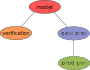
\includegraphics[width=0.4\columnwidth]{cycle1}
  \caption{First stage workflow}
  \label{fig:cycle1}
\end{figure}

The scenario presented in Figure \ref{fig:cycle-io} shows the same cycle of Figure \ref{fig:cycle1}, but the extended information about datasets is introduced.
In this picture, we have the tasks dependencies, and we explicit the datasets dependencies regarding the tasks that generated them.
The way data moves through tasks is by creating datasets to pass on the information, including filename and storage destination. The datasets produced by every task are coded in the workflow scripts before Cylc evaluation, and it is just replicated by this tool. The tasks can create a different number of datasets, and these datasets may be necessary for the immediate next task in the current cycle, or tasks in different cycles.

\begin{figure}[H]
  \centering
  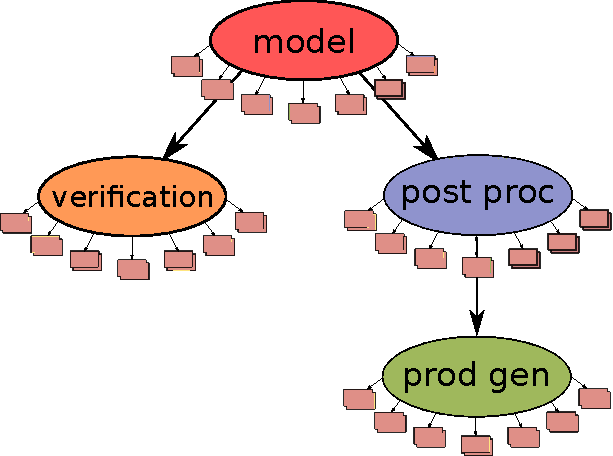
\includegraphics[width=0.6\columnwidth]{cycle-io}
  \caption{First stage workflow including datasets}
  \label{fig:cycle-io}
\end{figure}

Figure \ref{fig:cycle-io-dep} now introduces one example of dependencies among the datasets and tasks: datasets colours indicate which task will use their information and datasets in yellow represent information that will be used in a different cycle. The tricky part when we consider only tasks and not the datasets in the workflow is that it may lead to the false impression that the tasks only depend on the immediately previous one. Note, for instance, that one dataset produced by Task \textbf{model} is later used in Task \textbf{prod\,gen}. That is not an immediate conclusion when we analyse just the arrows for the dependencies. It is clear that Task \textbf{model} is a dependency for Task \textbf{post\,prod}, which is then a dependency for Task \textbf{prod\,gen}. Still, the crucial information here is that any dataset currently being used in the current cycle can also be used later. From the figure we can also see that Task \textbf{model} will generate one dataset for Task \textbf{post\,proc}, one dataset for Task \textbf{prod\,gen}, two datasets for Task \textbf{verification}, and three datasets for a later cycle.
The access to this information before the process starts can be used to optimise how these datasets will be stored during the workflow. This information today is static and manual, leaving opportunities for automatisation and optimisations open.
The idea here is to embrace the concept that tasks dependencies are really datasets dependencies. Once we can insert the datasets explicitly in the workflow, it is easier to see that many optimisations regarding storage can be made.

\begin{figure}[H]
  \centering
  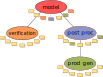
\includegraphics[width=0.6\columnwidth]{cycle-io-dep}
  \caption{First stage workflow including datasets and dependencies}
  \label{fig:cycle-io-dep}
\end{figure}

Figure \ref{fig:cycle-4} exemplifies another restriction of the way current workflows are being generated. Assume you have, for instance, four cycles of the model you are running. Because the scripts for the workflow consider individual tasks, the datasets generated by them are placed at the same storage type every time. That happens because all datasets generated by Task \textbf{model} will be used by Task \textbf{post\,prod}, so they should stay "closer" when thinking about memory. However, although this decision is based on an optimised concept, it still restricts the way the system deals with the datasets and optimisations that are not made thinking only about the local structure.

\begin{figure}[H]
  \centering
  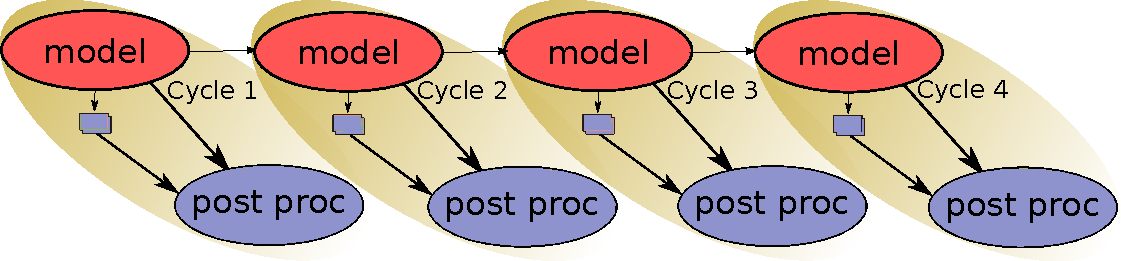
\includegraphics[width=0.8\columnwidth]{cycle-4}
  \caption{Four stages workflow example}
  \label{fig:cycle-4}
\end{figure}

Datasets generated by Task \textbf{A} and used by Task \textbf{B} will have the same physical location in the system because there is one fixed script responsible for setting the configuration. Again, such configuration was done manually and with restricted information about the storage and system architecture. It would be interesting to explore the options for the datasets and have them placed in different storage systems. If the lifetime of such dataset is, for instance, two cycles, alternate the datasets into two scratch dataset systems is something that would be a simple job for a tool working on generating filenames and storage. However, manually, that implies at having at least two scripts with information about the different storage and extra work to have better utilisation of the available resources.

The information about the system architecture can be provided in advance as a configuration file, and we can use monitoring to identify the I/O patterns for a specific workflow. For that, all we need is to run one cycle of the workflow and detect the patterns associated with it. For this purpose, we intend to use Machine Learning to identify the patterns and adapt the workflow in case of unexpected situations (the system is down, nodes are unresponsive, etc.).
With this separation of concepts, we can abstract from the workflow what is essential and has to be provided by the user and what a machine should optimise to ensure that the resources available are being used smartly. Every time parameters are manually tuned, that has a room from improvement by using automatised decision making. And Machine Learning has been proven effective in replacing human-beings in several problems.

Optimisations we can envision about the I/O are related to the life cycle of datasets and the placement of such datasets into specific memory according to their utilisation. What happens in most current workflows is that usually, they use only two types of file systems: \textbf{work} and \textbf{scratch}. When a task is set to computing, the corresponding dataset is moved to \textbf{scratch}, processed, and the resulting datasets are transferred back to \textbf{work}. If the \textbf{scratch} filesystem achieves its capacity, then the datasets move back to \textbf{work} and keep running the task until it is finished. If the I/O planning is made a priori, this situation can be avoided.
In addition to the file systems described, many supercomputers also have available for the user \textbf{scratch2} fyle systems (sometimes local and global). Therefore, in a real scenario, if the architecture of the machine is known, we can better use its resources.

\section{Conclusions}
\label{sec:conclusions}

Now:
\begin{enumerate}
  \item user runs Cylc to start a suite
  \item Cylc parses the suite file, generate dependencies and generate a schedule for the execution
  \item Once a task can be executed because dependencies are ready: Cylc generates on the fly a Slurm script with the required metadata for SLURM and invoking the user-defined script for that task and then runs Slurm to queue the script
  \item Slurm queues the task, and once the task is ready to be dispatched it is started on the supercomputer
  \item The shell-script executes the users-provided instructions, some of those are to generate file names using Cylc and the variables that are generated by Cylc. These filenames use templates provided by the user that defines the storage location to be used.
  \item User-specified applications run taking the filenames as instructed.
  The application may use NetCDF or XIOS to perform the I/O.

\end{enumerate}

Our Plan:

\begin{enumerate}
  \item user runs Cylc to start a suite.
  \item Cylc parses the suite file, generate dependencies and generate a schedule for the execution.

  Now, Cylc will call into EWIOScheduler to potentially reprioritise the order of execution of tasks.
  The EWIOScheduler will read the suite file and the suite-io.rc file to make suggestions but won't enforce anything.

  \item Once a task can be executed because dependencies are ready: Cylc generates on the fly a Slurm script with the required metadata for SLURM and invoking the user-defined script for that task.

  Potentially, Cylc will change the metadata of the script telling Slurm to place a job on the same nodes as a previous job to reuse local data.
  Potentially, Cylc may also add as metadata information to migrate data.

  Then runs Slurm to queue the task.

  \item Slurm queues the task, and once the task is ready to be dispatched it is started on the supercomputer

  If migration has to be performed before or after a job is run, it would do so.

  \item The shell-script executes the users-provided instructions, some of those are to generate file names using Cylc and the variables that are generated by Cylc.
  These filenames use templates provided by the user that defines the storage location to be used.

  The way filenames are generated now slightly different, using a new command that then uses ESWIOSchedule.
  The guy reads the suite file(s) and generates information for ESDM where to prioritise to place or access data. The filename hence encoded additional information.
  Potentially, we generate an esdm.conf file to reflect the specific hardware we want to use.

  \item User-specified applications run taking the filenames as instructed.
    The application may use NetCDF, XIOS

    OR ESDM

    to perform the I/O.

Knowing the potential targets, ESDM loads the system configuration to schedule application-local I/O.
  The application uses ESDM with the script filename, ESDM extracts the long-term schedule information and considers it during "application-local" I/O scheduling.

  \item A data management service may run and purge or migrate data according to user-specifications of the information life cycle.

\end{enumerate}

\begin{comment}

and computer-aided Research Development and Engineering (RD\&E)


and also on small-scale systems.

For example, Big data tools integrate computing and storage capabilities into a holistic solution demonstrating the benefit of tight integrating for data-driven workflows.

%-- the quality of service features available in hardware is rarely used.

Cloud definition of desired state and contracts.

Indeed many research prototypes address subproblems
* But not all aspects together
* Competing approaches; the standardisation we describe here does not compete!

In this paper, we purposely do not mention too many of the ongoing RD\&E in storage and computing.

To wrap up, NGI provides a high-level view on data and processing on heterogeneous platforms while shielding the user from execution details.

Open ...

%Kubernetes

\begin{description}

\item{NFS} Relatively slow, persistent file system - Nightly incremental backups

\item{Lustre} Large, fast distributed scratch file system - No backups

\url{https://info.hpc.sussex.ac.uk/hpc-guide/storage.html}

\end{description}

%, and data products are generated, which are processes that are executed outside of the first simulation.

\end{comment}



\section{Challenges and Limitations}
\label{sec:challenges}
The current HPC environment faces several challenges and limitations concerning the execution of data-driven workflows.

\begin{description}
\item[Explicit Workflows]

Typically, as part of shell scripts, users explicitly encode data processing workflows as a sequence of steps consisting of input, computing, and output.
The computing-intense parts (jobs) and their dependencies are managed by a cluster resource manager that dispatches them.
These loosely coupled workflows require that intermediate results are stored on persistent storage to be used by the next task.
Data transfer, however, needs a dominant fraction of energy compared to computation favouring offloading of computation to storage.

\item[Suboptimal Storage Tiering]

Organising the data placement on storage tiers is typically performed manually by the developer/user or via policies, leading to suboptimal optimisations. On top of that, it is a tedious and error-prone task.

Manual tiering requires the user or application to control the data placement, i.e., storing data (typically in the form of files) on a particular storage system and, usually, moving data between storage by using scripts.
One limitation here is that decisions about how data structures are mapped and packaged into files are made once by the producing application, and cannot be changed without manual intervention by a downstream application.

A policy system (e.g. burst buffer) aims to simplify the data movement for the user, but typically migrates objects in the coarse granularity of files.
However, the semantical information that can be used by a policy system to make decisions is limited, e.g., data location, file extension, age of the file, etc.

Any hard-coded decision has significant implications for the performance of both applications and systems because the optimal choices about file size and content may be very different for the data production and any subsequent data analysis phase.
In any case, data migration needs resources from the source and the target storage system to copy data.
Thus, to avoid extra manual work and decisions, it is preferable to direct data to locations where it can be stored and directly used by subsequent workflows -- at best, coupling the data source producing data with a data consumer to prevent storing intermediate products on persistent storage.

\item[Task and Data Equality]

All tasks and data products are handled identically by a HPC system, meaning there is no differentiation between individual jobs and data products.
This lack of hierarchy is problematic, as different use cases may not only differ in priority and deadline, but the computing speed usually depends on the critical path of the execution.

This problem is even more severe for data products: a storage system provides a single level of performance and resilience and performance for stored files.
Theoretically, different fault-tolerance and performance policies can be realised with varying storage systems and using management policies.
However, these policies would be coarse-grained and would not account for the priority of the workflow and, most importantly, the value of data.
The importance of data depends on aspects like costs to reproduce the data (can it be reproduced easily), the type of the experiment (test run, production run) and runtime constraints for the overall and potential crucial workflow.
While value and priority should influence fault-tolerance strategies and imply the quality of service for performance and availability, in practice, this is not the case as the storage just sees blocks and files.

\item[Manual Optimisation]

Utilising the computing and storage characteristics of a heterogeneous environment as depicted in \Cref{fig:heterogeneous} is challenging.
Even within a single data centre, utilising homogeneous storage and computing infrastructure efficiently is complex for experts and needs manual definition.
The efficient management of data and computing capabilities in a heterogeneous environment and
how the execution of individual tasks from workflows may benefit from alternative hardware architectures and infrastructures
are still unresolved questions.

The optimisation of a single parallel job already is quite challenging.
To make optimal use of available features, programmers and users are forced to think about technical aspects and terms, e.g., setting low-level MPI hints for file striping, while they understand their workflow.
Similarly, efficient data placement is complex. But a specific workflow combined with manual optimisation is the root-cause of subsequent problems, and it must be avoided and replaced with automated and optimised decisions.

Manual and hard-coded workflows cannot handle changes in the environment and are error-prone.
Therefore, users must be able to express their workflows in an abstract fashion that allows the system to generate (near-)optimal execution plans and monitor their execution.

\end{description}

\section{Vision}

Our vision for the problems described in the first sections is a new approach for data management and data-driven computation.


\begin{description}
\item[Workflow Specification]

The user defines a workflow describing the intentions of data manipulation and the data lifecycle, including manual (user) involvement in the data processing.
The definition of constraints, for instance, deadlines for the generation of the final data products (insight), can also be included.
Workflows can be defined using arbitrary tools, including Python.
Note that a user will not provide an accurate mapping to system or infrastructure, but expects that the system derives an optimised execution plan that covers heterogeneous infrastructures.
It does not matter where data is processed and how and where information is stored, but only that the desired result is computed with all constraints met.
Workflows and data lineage of data products are recorded and can be inspected by the user upon demand, allowing reproduction and validation of the correct execution of experiments.

\item[Smart Scheduling]

Supplied with user workflows and their characteristics, the system derives execution plans for the computation and make data placement decisions that aim to utilise the available hardware resources efficiently.
As the API is in charge of both tasks, it may decide to trade computation and storage capacity considering characteristics as costs and energy consumption, for example. Additionally, it can enable automatic recomputation of intermediate states utilising virtualisation and container technologies.
Similarly, the scheduler may decide to couple subsequent steps of a workflow directly without storing intermediate data products on persistent storage.
Data might be replicated but enables the system to rerun parts of the workflow in case of a data loss.

Automatic scheduling is key to efficient processing and will allow constant improvement without forcing the user to adjust their workflows.
In most cases, individual resources are not used exclusively by a single task, but QoS methods ensure that constraints of workflows are met.
Note that this is a significant change for HPC environments, as computing resources are typically dedicated to specific jobs.

\end{description}

\bibliographystyle{alpha}
\bibliography{paper}

\end{document}
